\index{stochastic gradient descent}
\index{SGD}
\chapter{SGD \& Modern Optimizers}
\newthought{THE Engine of Modern Deep Learning}


% ==============================================================================================
% INTRODUCTION BLOCK

\section{The Why}
\index{stochastic optimization}

\newthought{Throughout this course,} we've seen that gradient-based optimization requires computing:
\begin{equation}
    \nabla L(\theta) = \frac{1}{n} \sum_{i=1}^{n} \nabla \ell(\theta, x_i)
\end{equation}

For ImageNet with $n = 1.2$ million images and a ResNet with $p = 25$ million parameters, each gradient computation costs $\sim 3 \times 10^{13}$ operations. At 10 TFLOPS, that's $\sim 3$ seconds per gradient step.

\newthought{Training requires} tens of thousands of gradient steps. At 3 seconds each, that's days of training---just for one hyperparameter setting!

\marginnote{\newthought{The insight:} The gradient is an \emph{expectation}. We can estimate expectations with random samples. This is Monte Carlo estimation applied to optimization.}

\newthought{Stochastic Gradient Descent (SGD)} is the solution:
\begin{itemize}
    \item Approximate the full gradient with a random mini-batch
    \item Each update costs $O(b)$ instead of $O(n)$, where $b \ll n$
    \item More updates in the same time $\Rightarrow$ faster convergence in wall-clock time
\end{itemize}

\newthought{SGD + Backpropagation = The engine of modern AI.} Every neural network you've ever used was trained with some variant of SGD. Understanding it deeply means understanding how deep learning works.

\newthought{In machine learning and artificial intelligence:}
\begin{itemize}
    \item \texttt{loss.backward()} computes $\nabla \ell(\theta, x_{\text{batch}})$
    \item \texttt{optimizer.step()} performs the SGD (or Adam) update
    \item Learning rate schedules, momentum, Adam---all are refinements of this core idea
\end{itemize}



\newpage
\subsection{Hands On Experience}
\index{hands-on}
\index{mini-batch}

\newthought{Consider minimizing} $L(\theta) = \frac{1}{4}\sum_{i=1}^{4} (x_i - \theta)^2$ where $x = [1, 3, 5, 7]$.

The optimal $\theta^* = \frac{1+3+5+7}{4} = 4$.

\vspace{1em}
\newthought{Full gradient descent} from $\theta_0 = 0$ with $\alpha = 0.25$:
\begin{align*}
    \nabla L(0) &= \frac{1}{4}[2(0-1) + 2(0-3) + 2(0-5) + 2(0-7)] = \frac{1}{4}(-32) = -8 \\
    \theta_1 &= 0 - 0.25 \cdot (-8) = 2
\end{align*}

Each step uses all 4 data points.

\vspace{1em}
\newthought{Stochastic gradient descent} from $\theta_0 = 0$ with $\alpha = 0.25$, batch size 1:

\marginnote{\newthought{The key property:} $\mathbb{E}[\nabla \ell(\theta, x_i)] = \nabla L(\theta)$. The stochastic gradient is an \emph{unbiased estimate} of the true gradient.}

Pick random sample $x_2 = 3$:
\begin{align*}
    \nabla \ell(0, x_2) &= 2(0-3) = -6 \\
    \theta_1 &= 0 - 0.25 \cdot (-6) = 1.5
\end{align*}

Pick random sample $x_4 = 7$:
\begin{align*}
    \nabla \ell(1.5, x_4) &= 2(1.5-7) = -11 \\
    \theta_2 &= 1.5 - 0.25 \cdot (-11) = 4.25
\end{align*}

After 2 SGD updates (2 sample evaluations), we're at $\theta = 4.25$.

After 1 full GD update (4 sample evaluations), we're at $\theta = 2$.

\newthought{SGD made more progress} with the same compute budget!



\vspace{2.5em}
\newthought{The Learning Objectives} of this chapter aim at providing you with the abilities to:
\begin{itemize}
    \item Derive and implement SGD from first principles
    \item Understand momentum and why it accelerates convergence
    \item Explain adaptive learning rate methods (AdaGrad, RMSprop, Adam)
    \item Apply learning rate schedules in practice
    \item Connect SGD theory to practical deep learning training
\end{itemize}




% ==============================================================================================
% MAIN THEORY BLOCK


%% ---- TOPIC 3: Newton's Method in Multiple Dimensions ----

\newpage

\section{Newton's Method in Multiple Dimensions}
\index{multivariate Newton} \index{Jacobian} \index{Hessian}

\newthought{So far,} we have seen Newton's method for optimization in 1D. Now we extend to systems of equations in multiple dimensions. Consider Shekel's foxholes in 2D:

\begin{equation}
    f(x, y) = -\sum_{i=1}^{m} \frac{c_i}{(x - a_i)^2 + (y - b_i)^2 + r_i}
\end{equation}

\begin{figure}[h]
    \centering
    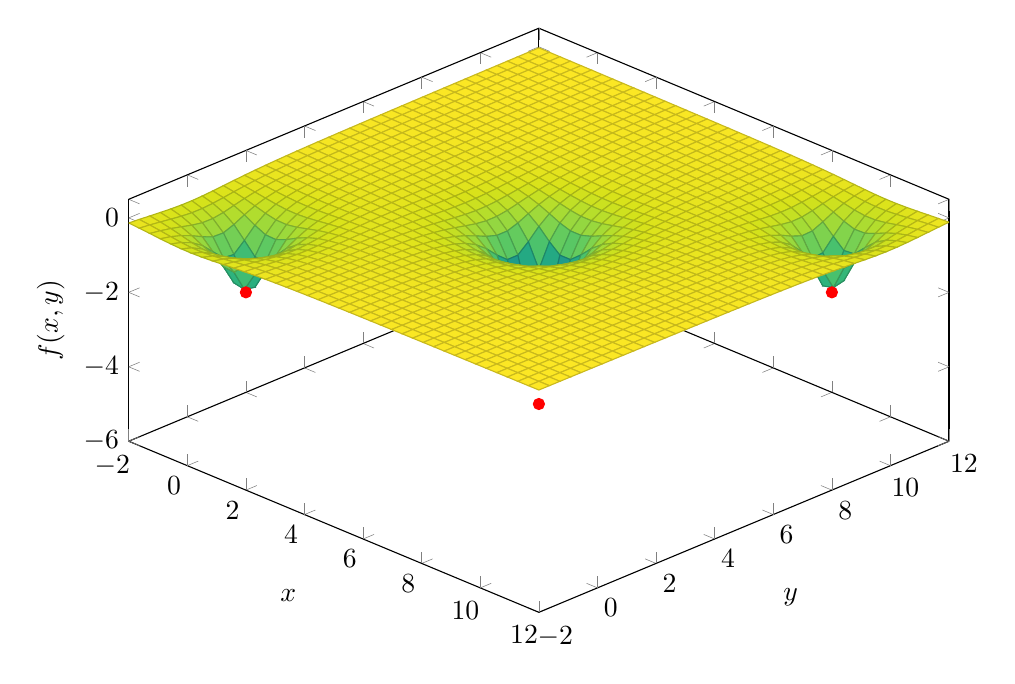
\begin{tikzpicture}
        \begin{axis}[
            width=12cm,
            height=9cm,
            view={45}{45},
            xlabel={$x$},
            ylabel={$y$},
            zlabel={$f(x,y)$},
            domain=-2:12,
            y domain=-2:12,
            samples=40,
            zmin=-6, zmax=0.5,
        ]
        \addplot3[
            surf,
            colormap/viridis,
        ] {-1/((x-0)^2 + (y-0)^2 + 0.5) - 1.5/((x-5)^2 + (y-5)^2 + 0.3) - 0.8/((x-10)^2 + (y-10)^2 + 0.4)};

        % Mark the three foxholes
        \addplot3[only marks, mark=*, mark size=2pt, color=red] coordinates {
            (0, 0, -2)
            (5, 5, -5)
            (10, 10, -2)
        };
        \end{axis}
    \end{tikzpicture}
    \caption{Shekel's foxholes in 2D with three valleys. The deepest valley at $(x,y) = (5,5)$ is the global minimum. Local optimization from different starting regions converges to different minima.}
    \label{fig:shekel_foxholes_2d}
\end{figure}

\newthought{For optimization} of this 2D function, we need the gradient and Hessian. For a single foxhole term $-c_i / ((x-a_i)^2 + (y-b_i)^2 + r_i)$, let $d_i^2 = (x-a_i)^2 + (y-b_i)^2 + r_i$. Then:
\begin{equation}
    \nabla f = \sum_{i=1}^{m} \frac{2c_i}{d_i^4} \begin{pmatrix} x - a_i \\ y - b_i \end{pmatrix}, \qquad
    \mathbf{H} = \sum_{i=1}^{m} \frac{2c_i}{d_i^4} \left[ \mathbf{I} - \frac{4}{d_i^2} \begin{pmatrix} x-a_i \\ y-b_i \end{pmatrix} \begin{pmatrix} x-a_i & y-b_i \end{pmatrix} \right]
\end{equation}

These are the concrete objects that Newton's method uses to navigate the 2D landscape---the gradient points toward steeper descent, and the Hessian captures how the curvature changes in each direction.

\newthought{The $n$-dimensional generalization.} In 1D, Newton for optimization uses $g''(x)$. In $n$ dimensions, the second derivative becomes the \textbf{Hessian matrix} $\mathbf{H}$:
\begin{equation}
    H_{ij} = \frac{\partial^2 g}{\partial x_i \, \partial x_j}
\end{equation}

and Newton's method for optimization becomes:
\begin{equation}
    \mathbf{x}_{n+1} = \mathbf{x}_n - \mathbf{H}(\mathbf{x}_n)^{-1} \nabla g(\mathbf{x}_n)
\end{equation}

\marginnote{\newthought{The Hessian} for a neural network with $p$ parameters is a $p \times p$ matrix. For GPT-3 with 175B parameters, that's $175\text{B} \times 175\text{B} \approx 10^{22}$ entries---clearly impossible to store or invert.}

The second derivative test also generalizes: if all eigenvalues of $\mathbf{H}(x^*)$ are positive (positive definite), we have a minimum; if all are negative, a maximum; if mixed signs, a saddle point. Saddle points are especially common in high-dimensional optimization and can slow convergence significantly.

\vspace{1em}
\newthought{Why gradient descent instead of Newton?}

\begin{table*}[ht]
\centering
\begin{tabular}{p{0.20\textwidth}p{0.28\textwidth}p{0.28\textwidth}}
\toprule
\textbf{Aspect} & \textbf{Newton} & \textbf{Gradient Descent} \\
\midrule
Per-iteration cost & $O(n^3)$ & $O(n)$ \\
Memory & $O(n^2)$ & $O(n)$ \\
Convergence & Quadratic & Linear \\
Step size & Auto-adapted & Manual tuning \\
\bottomrule
\end{tabular}
\vspace{2em}
\caption{Newton's method vs.\ gradient descent: Newton converges faster but is infeasible for large-scale problems.}
\label{tab:newton_vs_gd}
\end{table*}

\vspace{1em}
For $n = 10$ parameters, Newton wins. For $n = 10^8$ parameters (typical DNN), gradient descent is the only feasible option.

\newthought{Gradient descent is Newton with $\mathbf{H} \approx \mathbf{I}$:}
\begin{equation}
    \mathbf{x}_{n+1} = \mathbf{x}_n - \alpha \nabla f(\mathbf{x}_n)
\end{equation}

The learning rate $\alpha$ replaces the curvature information we're ignoring.


\subsection{The Jacobian and Multivariate Newton}

\newthought{Many problems involve systems} of equations. Consider finding $\mathbf{x}^*$ such that:
\begin{equation}
    \mathbf{F}(\mathbf{x}) = \mathbf{0}
\end{equation}
where $\mathbf{F}: \mathbb{R}^n \to \mathbb{R}^n$ and $\mathbf{x} \in \mathbb{R}^n$.

\marginnote{\newthought{In neural networks,} training involves solving $\nabla L(\theta) = 0$, a system of millions of equations in millions of variables.}

\newthought{The Jacobian matrix} generalizes the derivative to multiple dimensions:
\begin{equation}
    \mathbf{J}(\mathbf{x}) = \begin{bmatrix}
        \frac{\partial F_1}{\partial x_1} & \cdots & \frac{\partial F_1}{\partial x_n} \\
        \vdots & \ddots & \vdots \\
        \frac{\partial F_n}{\partial x_1} & \cdots & \frac{\partial F_n}{\partial x_n}
    \end{bmatrix}
\end{equation}

\newthought{Multivariate Newton iteration:}
\begin{equation}
    \mathbf{x}_{n+1} = \mathbf{x}_n - \mathbf{J}(\mathbf{x}_n)^{-1} \mathbf{F}(\mathbf{x}_n)
\end{equation}

In practice, we solve the linear system $\mathbf{J}(\mathbf{x}_n) \mathbf{d} = -\mathbf{F}(\mathbf{x}_n)$ for $\mathbf{d}$, then update
$\mathbf{x}_{n+1} = \mathbf{x}_n + \mathbf{d}$.

\newthought{Connection to optimization:} For minimizing a scalar function $f(\mathbf{x})$, we set $\mathbf{F} = \nabla f$ and solve $\nabla f(\mathbf{x}) = \mathbf{0}$. The Jacobian of the gradient is precisely the Hessian: $\mathbf{J} = \mathbf{H}$. So multivariate Newton for root finding and Newton for optimization are the same framework---the optimization case is the special case where $\mathbf{F}$ is a gradient field.


\subsection{Example: 2D System}

\newthought{As a root-finding example,} consider finding the intersection of a circle and a line:
\begin{align}
    F_1(x, y) &= x^2 + y^2 - 4 = 0 \quad \text{(circle)} \\
    F_2(x, y) &= x - y = 0 \quad \text{(line)}
\end{align}

The Jacobian is:
\begin{equation}
    \mathbf{J} = \begin{bmatrix}
        2x & 2y \\
        1 & -1
    \end{bmatrix}
\end{equation}

Starting from $\mathbf{x}_0 = (1, 0)^T$:
\begin{align*}
    \mathbf{F}(\mathbf{x}_0) &= \begin{pmatrix} 1 + 0 - 4 \\ 1 - 0 \end{pmatrix} = \begin{pmatrix} -3 \\ 1 \end{pmatrix} \\
    \mathbf{J}(\mathbf{x}_0) &= \begin{bmatrix} 2 & 0 \\ 1 & -1 \end{bmatrix} \\
    \mathbf{J}^{-1} &= \begin{bmatrix} 0.5 & 0 \\ 0.5 & -1 \end{bmatrix} \\
    \mathbf{x}_1 &= \begin{pmatrix} 1 \\ 0 \end{pmatrix} - \begin{bmatrix} 0.5 & 0 \\ 0.5 & -1 \end{bmatrix} \begin{pmatrix} -3 \\ 1 \end{pmatrix} = \begin{pmatrix} 2.5 \\ -2.5 \end{pmatrix}
\end{align*}

After a few iterations: $\mathbf{x}^* \approx (\sqrt{2}, \sqrt{2})$.

\newthought{Note:} This is a root-finding problem ($\mathbf{F}(\mathbf{x}) = \mathbf{0}$), not an optimization problem. For optimization of a function $f(x,y)$, we would set $\mathbf{F} = \nabla f = ({\partial f}/{\partial x},\, {\partial f}/{\partial y})^T$ and the Jacobian would be the Hessian $\mathbf{H}$. The same Newton machinery applies---only the interpretation of $\mathbf{F}$ changes.



\newpage
\section{Stochastic Gradient Descent}
\index{stochastic gradient descent}

\subsection{From Full Gradient to Stochastic Gradient}
\index{gradient estimation}

\newthought{The expected loss} over a data distribution $p(x)$ is:
\begin{equation}
    L(\theta) = \mathbb{E}_{x \sim p}[\ell(\theta, x)] = \int \ell(\theta, x) p(x) dx
\end{equation}

\marginnote{\newthought{In practice,} we don't know $p(x)$. We approximate the expectation with the empirical mean over our dataset: $L(\theta) \approx \frac{1}{n}\sum_{i=1}^n \ell(\theta, x_i)$.}

\newthought{The gradient} of the expected loss:
\begin{equation}
    \nabla L(\theta) = \mathbb{E}_{x \sim p}[\nabla \ell(\theta, x)]
\end{equation}

\newthought{Key insight:} We can estimate this expectation by sampling!

\begin{equation}
    \nabla L(\theta) \approx g(\theta) = \frac{1}{|B|} \sum_{i \in B} \nabla \ell(\theta, x_i)
\end{equation}

where $B$ is a random mini-batch of size $|B| = b$.

\newthought{Properties of the stochastic gradient:}
\begin{itemize}
    \item \textbf{Unbiased:} $\mathbb{E}[g(\theta)] = \nabla L(\theta)$
    \item \textbf{Variance:} $\text{Var}(g) \propto \frac{1}{b}$ (larger batches $\Rightarrow$ lower variance)
    \item \textbf{Cost:} $O(b \cdot p)$ instead of $O(n \cdot p)$
\end{itemize}

\newthought{The SGD update:}
\begin{equation}
    \boxed{\theta_{t+1} = \theta_t - \alpha \cdot g_t}
\end{equation}

where $g_t = \frac{1}{|B_t|} \sum_{i \in B_t} \nabla \ell(\theta_t, x_i)$ and $B_t$ is a fresh random batch.

\begin{algorithm}[H]
\caption{Stochastic Gradient Descent (SGD)}
\begin{algorithmic}[1]
    \Require Initial parameters $\theta_0$, learning rate $\alpha$, batch size $b$, dataset $\mathcal{D}$
    \State $t \gets 0$
    \While{not converged}
        \State Sample mini-batch: $B_t \gets \text{random\_sample}(\mathcal{D}, b)$
        \State Compute stochastic gradient: $g_t \gets \frac{1}{b} \sum_{x \in B_t} \nabla \ell(\theta_t, x)$
        \State Update parameters: $\theta_{t+1} \gets \theta_t - \alpha \cdot g_t$
        \State $t \gets t + 1$
    \EndWhile
    \Return $\theta_t$
\end{algorithmic}
\end{algorithm}



\subsection{Convergence of SGD}
\index{SGD convergence}

\newthought{For convex functions,} SGD converges at rate $O(1/\sqrt{k})$:
\begin{equation}
    \mathbb{E}[L(\theta_k)] - L(\theta^*) \leq \frac{C}{\sqrt{k}}
\end{equation}

\marginnote{\newthought{Sublinear convergence} is slower than linear (GD), but SGD does many more iterations in the same time, so wall-clock time can be faster.}

This is \emph{sublinear}---slower than GD's linear convergence. But:
\begin{itemize}
    \item Each SGD iteration is $n/b$ times cheaper
    \item For $n = 10^6$, $b = 100$: SGD does 10,000 iterations in the time GD does 1
    \item Total progress: SGD often wins in wall-clock time
\end{itemize}

\newthought{For non-convex functions} (neural networks):
\begin{itemize}
    \item Theory is less clean, but SGD still works remarkably well
    \item The noise helps escape sharp local minima
    \item Implicit regularization: SGD prefers ``flat'' minima that generalize better
\end{itemize}



\subsection{The Role of Batch Size}
\index{batch size}

\begin{figure}[h]
    \centering
    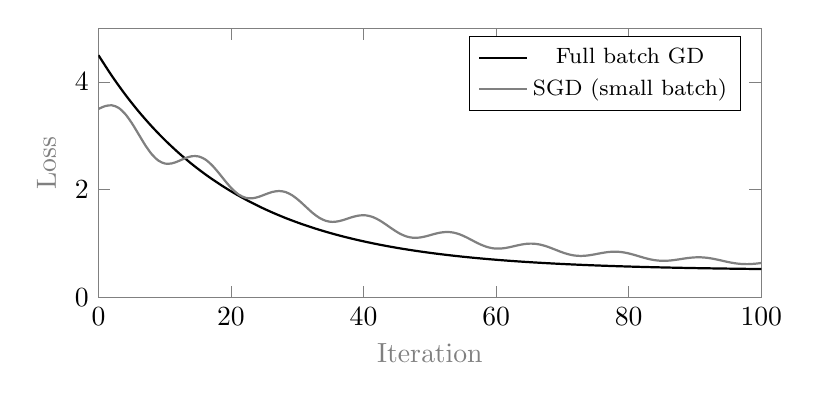
\begin{tikzpicture}
        \begin{axis}[
            width=10cm,
            height=5cm,
            xlabel={Iteration},
            ylabel={Loss},
            xmin=0, xmax=100,
            ymin=0, ymax=5,
            tick style={gray},
            label style={gray},
            axis line style={gray},
            legend pos=north east,
            legend style={font=\footnotesize},
        ]
        % Full batch GD (smooth)
        \addplot[black, thick, smooth, domain=0:100, samples=50] {4*exp(-0.05*x) + 0.5};
        \addlegendentry{Full batch GD}
        % SGD with small batch (noisy)
        \addplot[gray, thick, smooth, domain=0:100, samples=100] {3*exp(-0.03*x) + 0.5 + 0.3*sin(deg(x*0.5))*exp(-0.02*x)};
        \addlegendentry{SGD (small batch)}
        \end{axis}
    \end{tikzpicture}
    \caption{SGD with small batches is noisier but often reaches good solutions faster due to regularization effects.}
    \label{fig:sgd_vs_gd}
\end{figure}

\newthought{Small batches} ($b = 32$--$128$):
\begin{itemize}
    \item High variance $\Rightarrow$ noisy updates
    \item Good exploration, implicit regularization
    \item Often generalizes better
\end{itemize}

\newthought{Large batches} ($b = 1024$--$32768$):
\begin{itemize}
    \item Low variance $\Rightarrow$ smoother updates
    \item Better hardware utilization (GPU parallelism)
    \item May need learning rate adjustment
\end{itemize}

\marginnote{\newthought{Linear scaling rule:} When you increase batch size by $k\times$, increase learning rate by $k\times$ (up to a point). This maintains similar training dynamics.}




\newpage
\section{Momentum}
\index{momentum}

\newthought{Problem with vanilla SGD:} Oscillates in narrow valleys, slow progress along the valley floor.

\begin{figure}[h]
    \centering
    \begin{tikzpicture}
        % Draw contour lines of an elongated quadratic
        \begin{axis}[
            width=8cm,
            height=5cm,
            xlabel={$\theta_1$},
            ylabel={$\theta_2$},
            xmin=-3, xmax=3,
            ymin=-2, ymax=2,
            tick style={gray},
            label style={gray},
            axis equal,
            view={0}{90},
        ]
        % Contour plot
        \addplot[contour gnuplot={number=8, labels=false}, thick, gray]
            {0.1*x^2 + 2*y^2};
        % SGD path (oscillating)
        \addplot[black, thick, ->] coordinates {
            (-2.5, 1.5) (-2.2, -0.8) (-1.8, 0.5) (-1.4, -0.3) (-1.0, 0.15) (-0.6, -0.08) (-0.3, 0.04) (0, 0)
        };
        \end{axis}
    \end{tikzpicture}
    \caption{SGD oscillates across the narrow valley while making slow progress along it.}
    \label{fig:sgd_oscillation}
\end{figure}

\newthought{The idea:} Add ``momentum'' like a ball rolling downhill. The ball accumulates velocity and doesn't change direction instantly.

\newthought{Momentum update:}
\begin{align}
    v_t &= \beta v_{t-1} + g_t \\
    \theta_{t+1} &= \theta_t - \alpha v_t
\end{align}

where $\beta \in [0, 1)$ is the momentum coefficient (typically $\beta = 0.9$).

\marginnote{\newthought{Physical intuition:} $v_t$ is velocity, $g_t$ is acceleration (force), $\beta$ is friction. The ball builds up speed in consistent directions and averages out oscillations.}

\newthought{Why momentum helps:}
\begin{itemize}
    \item Gradients in the ``valley direction'' accumulate: $v_t \approx g/(1-\beta)$
    \item Oscillating gradients cancel out over time
    \item Effectively takes larger steps in low-curvature directions
\end{itemize}

\newthought{Nesterov momentum} (look-ahead):
\begin{align}
    v_t &= \beta v_{t-1} + \nabla L(\theta_t - \alpha \beta v_{t-1}) \\
    \theta_{t+1} &= \theta_t - \alpha v_t
\end{align}

Evaluate the gradient at the ``look-ahead'' position. Often slightly better in practice.




\newpage
\section{Adaptive Learning Rates}
\index{adaptive learning rate}

\newthought{Problem:} Different parameters may need different learning rates.
\begin{itemize}
    \item Frequent features: gradients are large, need small LR
    \item Rare features: gradients are small, need large LR
\end{itemize}

\subsection{AdaGrad}
\index{AdaGrad}

\newthought{Idea:} Divide by cumulative sum of squared gradients.

\begin{align}
    s_t &= s_{t-1} + g_t^2 \quad \text{(element-wise)} \\
    \theta_{t+1} &= \theta_t - \frac{\alpha}{\sqrt{s_t} + \varepsilon} \cdot g_t
\end{align}

\marginnote{\newthought{$\varepsilon \approx 10^{-8}$} prevents division by zero. This tiny constant appears in all adaptive methods.}

\newthought{Properties:}
\begin{itemize}
    \item Large gradients $\Rightarrow$ large $s_t$ $\Rightarrow$ small effective LR
    \item Small gradients $\Rightarrow$ small $s_t$ $\Rightarrow$ large effective LR
    \item Problem: $s_t$ only grows $\Rightarrow$ LR eventually becomes tiny
\end{itemize}


\subsection{RMSprop}
\index{RMSprop}

\newthought{Fix AdaGrad's problem:} Use exponential moving average instead of cumulative sum.

\begin{align}
    s_t &= \beta_2 s_{t-1} + (1 - \beta_2) g_t^2 \\
    \theta_{t+1} &= \theta_t - \frac{\alpha}{\sqrt{s_t} + \varepsilon} \cdot g_t
\end{align}

Typically $\beta_2 = 0.99$. The ``memory'' decays, so old gradients are forgotten.


\subsection{Adam}
\index{Adam}

\newthought{Adam = Momentum + RMSprop.} The most popular optimizer in deep learning.

\begin{align}
    m_t &= \beta_1 m_{t-1} + (1 - \beta_1) g_t \quad \text{(first moment / momentum)} \\
    v_t &= \beta_2 v_{t-1} + (1 - \beta_2) g_t^2 \quad \text{(second moment / variance)} \\
    \hat{m}_t &= \frac{m_t}{1 - \beta_1^t} \quad \text{(bias correction)} \\
    \hat{v}_t &= \frac{v_t}{1 - \beta_2^t} \quad \text{(bias correction)} \\
    \theta_{t+1} &= \theta_t - \alpha \frac{\hat{m}_t}{\sqrt{\hat{v}_t} + \varepsilon}
\end{align}

\marginnote{\newthought{Bias correction:} Since $m_0 = v_0 = 0$, early estimates are biased toward zero. The correction $1/(1-\beta^t)$ compensates.}

\begin{algorithm}[H]
\caption{Adam Optimizer}
\begin{algorithmic}[1]
    \Require Initial parameters $\theta_0$, learning rate $\alpha$, decay rates $\beta_1, \beta_2$, $\varepsilon = 10^{-8}$
    \State Initialize: $m_0 \gets 0$, $v_0 \gets 0$, $t \gets 0$
    \While{not converged}
        \State $t \gets t + 1$
        \State Compute gradient: $g_t \gets \nabla L(\theta_{t-1})$
        \State Update first moment: $m_t \gets \beta_1 m_{t-1} + (1-\beta_1) g_t$
        \State Update second moment: $v_t \gets \beta_2 v_{t-1} + (1-\beta_2) g_t^2$
        \State Bias-correct first moment: $\hat{m}_t \gets m_t / (1 - \beta_1^t)$
        \State Bias-correct second moment: $\hat{v}_t \gets v_t / (1 - \beta_2^t)$
        \State Update parameters: $\theta_t \gets \theta_{t-1} - \alpha \cdot \hat{m}_t / (\sqrt{\hat{v}_t} + \varepsilon)$
    \EndWhile
    \Return $\theta_t$
\end{algorithmic}
\end{algorithm}

\newthought{Default hyperparameters:}
\begin{itemize}
    \item $\alpha = 0.001$ (learning rate)
    \item $\beta_1 = 0.9$ (momentum)
    \item $\beta_2 = 0.999$ (second moment decay)
    \item $\varepsilon = 10^{-8}$ (numerical stability)
\end{itemize}

\newthought{AdamW} adds weight decay (L2 regularization) directly to the update:
\begin{equation}
    \theta_{t+1} = \theta_t - \alpha \left( \frac{\hat{m}_t}{\sqrt{\hat{v}_t} + \varepsilon} + \lambda \theta_t \right)
\end{equation}

This is the default optimizer for training transformers (BERT, GPT, etc.).




\newpage
\section{Learning Rate Schedules}
\index{learning rate schedule}

\newthought{Fixed learning rate} is rarely optimal. Common schedules:

\subsection{Step Decay}
\index{step decay}
Reduce LR by factor $\gamma$ every $k$ epochs:
\begin{equation}
    \alpha_t = \alpha_0 \cdot \gamma^{\lfloor t/k \rfloor}
\end{equation}

Example: $\alpha_0 = 0.1$, $\gamma = 0.1$, $k = 30$ epochs.

\subsection{Exponential Decay}
\index{exponential decay}
\begin{equation}
    \alpha_t = \alpha_0 \cdot e^{-\lambda t}
\end{equation}

\subsection{Cosine Annealing}
\index{cosine annealing}
\begin{equation}
    \alpha_t = \alpha_{\min} + \frac{1}{2}(\alpha_{\max} - \alpha_{\min})\left(1 + \cos\left(\frac{t}{T}\pi\right)\right)
\end{equation}

Smooth decay from $\alpha_{\max}$ to $\alpha_{\min}$ over $T$ steps.

\begin{figure}[h]
    \centering
    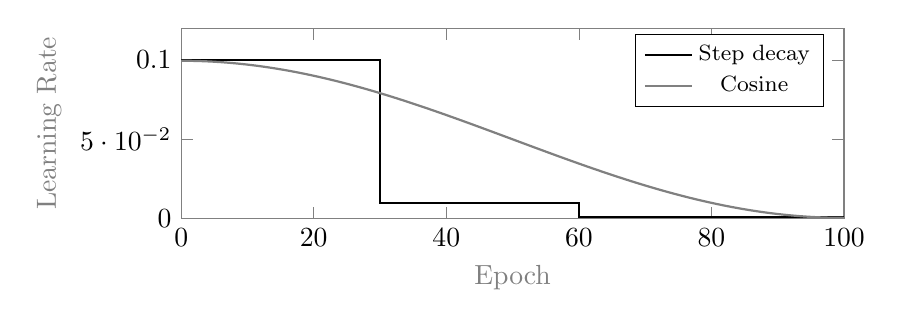
\begin{tikzpicture}
        \begin{axis}[
            width=10cm,
            height=4cm,
            xlabel={Epoch},
            ylabel={Learning Rate},
            xmin=0, xmax=100,
            ymin=0, ymax=0.12,
            tick style={gray},
            label style={gray},
            axis line style={gray},
            legend pos=north east,
            legend style={font=\footnotesize},
        ]
        % Step decay
        \addplot[black, thick] coordinates {
            (0, 0.1) (30, 0.1) (30, 0.01) (60, 0.01) (60, 0.001) (100, 0.001)
        };
        \addlegendentry{Step decay}
        % Cosine
        \addplot[gray, thick, smooth, domain=0:100, samples=100] {0.0005 + 0.0495*(1 + cos(deg(x*3.14159/100)))};
        \addlegendentry{Cosine}
        \end{axis}
    \end{tikzpicture}
    \caption{Step decay vs. cosine annealing learning rate schedules.}
    \label{fig:lr_schedules}
\end{figure}

\subsection{Warmup}
\index{warmup}

\marginnote{\newthought{Why warmup?} At initialization, the loss landscape may be poorly behaved. Small LR initially allows the optimizer to find a reasonable region before taking larger steps.}

\newthought{Critical for Transformers:} Start with small LR and increase linearly.

\begin{equation}
    \alpha_t = \begin{cases}
        \alpha_{\max} \cdot \frac{t}{T_{\text{warmup}}} & \text{if } t < T_{\text{warmup}} \\
        \text{schedule}(t) & \text{otherwise}
    \end{cases}
\end{equation}

Common: 1--10\% of training as warmup, then cosine decay.






% ==============================================================================================
% STUDENT ACTIVATION BLOCK

\newpage
\section{Examples \& Exercises}
\index{exercises}

\marginnote{\newthought{Code} can be found at \url{https://github.com/Quillstacks/lecturecode_numericalmethods.git}.}

\newthought{Exercise 1: SGD by hand.} Minimize $L(\theta) = \frac{1}{3}\sum_{i=1}^{3}(x_i - \theta)^2$ where $x = [0, 3, 6]$.

Starting from $\theta_0 = 0$, $\alpha = 0.2$:
\begin{enumerate}
    \item Compute one full gradient step
    \item Compute three SGD steps (one sample each)
    \item Compare final $\theta$ values
\end{enumerate}


\vspace{2em}
\newthought{Exercise 2: Momentum calculation.} With $\beta = 0.9$, $\alpha = 0.1$, compute 3 momentum updates.

Given gradient sequence $g_1 = 2$, $g_2 = 2$, $g_3 = 2$, starting from $v_0 = 0$, $\theta_0 = 0$:
\begin{align*}
    v_1 &= 0.9 \cdot 0 + 2 = 2 \\
    \theta_1 &= 0 - 0.1 \cdot 2 = -0.2 \\[6pt]
    v_2 &= 0.9 \cdot 2 + 2 = 3.8 \\
    \theta_2 &= -0.2 - 0.1 \cdot 3.8 = -0.58 \\[6pt]
    v_3 &= 0.9 \cdot 3.8 + 2 = 5.42 \\
    \theta_3 &= -0.58 - 0.1 \cdot 5.42 = -1.12
\end{align*}

Notice how velocity builds up when gradients are consistent!


\vspace{2em}
\newthought{Exercise 3: Adam step.} Compute one Adam update with $\alpha = 0.01$, $\beta_1 = 0.9$, $\beta_2 = 0.999$, $\varepsilon = 10^{-8}$.

Given $m_0 = 0$, $v_0 = 0$, $g_1 = 0.5$:
\begin{align*}
    m_1 &= 0.9 \cdot 0 + 0.1 \cdot 0.5 = 0.05 \\
    v_1 &= 0.999 \cdot 0 + 0.001 \cdot 0.25 = 0.00025 \\
    \hat{m}_1 &= 0.05 / (1 - 0.9) = 0.5 \\
    \hat{v}_1 &= 0.00025 / (1 - 0.999) = 0.25 \\
    \Delta\theta &= 0.01 \cdot 0.5 / (\sqrt{0.25} + 10^{-8}) = 0.01 \cdot 0.5 / 0.5 = 0.01
\end{align*}


\vspace{2em}
\newthought{Exercise 4: Batch size scaling.} You're training with batch size 64 and LR $\alpha = 0.01$. If you increase batch size to 256, what LR should you use according to the linear scaling rule?

\textit{Answer:} Scale by $256/64 = 4$, so use $\alpha = 0.04$.


\newpage
\section{Self-Reflection and Recap}
\index{recap}

\newthought{Self-Reflection} Questions to guide your understanding:
\begin{itemize}
    \item Why is the stochastic gradient an \emph{unbiased} estimate of the true gradient?
    \item How does SGD noise help escape sharp local minima?
    \item When would you choose Adam over SGD with momentum?
    \item Why is warmup critical for training Transformers?
    \item What's the trade-off between small and large batch sizes?
\end{itemize}

\newthought{Recap} of Key Concepts:
\begin{itemize}
    \item \textbf{SGD:} Approximate gradient with random mini-batch; $O(b)$ instead of $O(n)$.
    \item \textbf{Momentum:} Accumulate velocity to smooth oscillations and accelerate.
    \item \textbf{Adam:} Momentum + adaptive learning rates; the go-to optimizer.
    \item \textbf{Learning rate schedules:} Start high (or warmup), decay over training.
    \item \textbf{Batch size:} Smaller = more noise/regularization; larger = better hardware utilization.
\end{itemize}


\marginnote{\newthought{Teaser.} SGD can train one GPU efficiently. But GPT-4 has \textbf{1.8 trillion parameters} and trains on \textbf{trillions of tokens}. How do we \textbf{scale to this magnitude}?}

\newthought{From one GPU to thousands.} SGD makes training feasible, but modern models are too large for any single machine. In the next chapter, we'll study \emph{parallel and distributed computing}---how to split data and models across thousands of GPUs, and why understanding complexity and memory constraints is essential for training at scale.



%%%%%%%%%%%%%%%%%%%%%%%%%%%%%%%%%%%%%%%%%%%%%%%%%%%%%%%%%%%%%%%%%%%%%%%%%%%%%%
